%\begin{appendices}
%\addcontentsline{toc}{chapter}{Appendicies}

\appendix

\begingroup
\renewcommand{\cleardoublepage}{}
\renewcommand{\clearpage}{}
\chapter{Deterministic Annealing} \label{app:DA}
  The free energy analog is

  \[
    F = -T \sum \limits_i^{\text{\# tracks}} p_i \log \left( \sum \limits_k^{\text{\# vertices}} \rho_k \exp \left[ -\frac{\left(z_i^t - z_k^v\right)^2}{T (\sigma_i^z)^2} \right] \right)
  \]

  where $p_i$ is the weight of the track $i$, a measure of its quality from 0 to 1, $z_i^t$ and $z_k^v$ are the positions of the track $i$ and vertex $k$ along the beamline with $\sigma_i^z$ being the uncertainty in the position of the track, and $\rho_k$ is a measure of the vertex quality. The upshot of this method is that as the temperature T is reduced, the optimal number of vertices to accommodate the tracks begins to increase with each track getting its own vertex at $T=0$. The final number of vertices is set at special temperature of $T=4$, which  was identified as a good compromise between incorrect splitting and vertex resolution. A track $i$ is assigned a probability to come from a vertex $k$ by a Maxwell-Boltzmann distribution 

  \[ 
    p_{ik} = \frac{\rho_k \exp \left[ -\frac{\left(z_i^t - z_k^v\right)^2}{T (\sigma_i^z)^2} \right]} { \sum \limits_j^{\text{\# vertices}} \rho_{j} \exp \left[ -\frac{\left(z_i^t - z_j^v\right)^2}{T (\sigma_i^z)^2} \right]}. 
  \]

  The final vertex assignment is done by taking the highest probability vertex for each track at $T=1$.

\chapter{The motion of particles in a magnetic field} \label{app:sagitta}
\endgroup
  Magnetic fields can not change the magnitude of velocity for a charged particle due to the Lorentz force law containing a cross product that includes $\vec{v}$,

  \[
    \vec{F} = q\vec{v}\times\vec{B}.
  \]

  This means that a charged particle in a magnetic field feels an acceleration which attempts to turn it in a circle at constant velocity. It is well known that this type of centripetal acceleration must have magnitude $a = \frac{v^2}{r}$. Therefore, 

  \[
    \frac{mv^2}{r} = q\vec{v}\times\vec{B}
  \]

  by collecting terms, we can find the momentum of the particle in terms of the radius of rotation and the magnetic field

  \[
    p = qBr.
  \]

  This relationship still holds in the relativistic case when $p = mv \to \gamma mv$.

  \begin{figure}[h!]
    \centering
    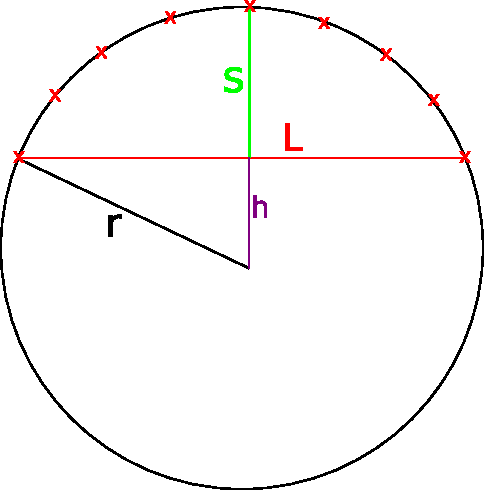
\includegraphics[width=.4\textwidth]{figures/Sagitta.pdf}
    \caption[The Sagitta of the circle.]{The Sagitta of the circle. The red x symbols represent where a particle detector might sample the position of a particle moving along the segment whose endpoints coincide with the chord $L$. The sagitta, $s$, is what is measured directly by detectors and used to estimate the momentum of charged particles in a magnetic field.}
    \label{fig:sagitta}
  \end{figure}

  The radius of motion caused by the magnetic field in a particle detector can not be measured directly. Particle detectors essentially sample the motion of the particle at various points along its trajectory. Figure \ref{fig:sagitta} shows an example of a circular arc which represents the trajectory of a charged particle, the red x symbols represent points where a hit was recorded by the detector. To get a measure of the radius of curvature, the sagitta of the track can be measured between the two terminal hits of the track, which is the maximal deviation of the particle's track from a straight line. 

  Using 
  \begin{align*}
    h+ s = r \text{ and} \\
    \left(\frac{L}{2}\right)^2 + h^2 = r^2
  \end{align*}

  yeilds

  \[
    s = r\left(1 - \sqrt{\left(1-\frac{L^2}{4r^2}\right)} \right).
  \]

  Expanding to first order about $\frac{L^2}{4r^2} = 0$, which is regulated by the momentum of the tracks, we can solve for $r$ to find

  \[
    r = \frac{L^2}{8s}.
  \]

  This can be replaced into the above expression for the momentum to yeild

  \[
    p=\frac{qBL^2}{8s}.
  \]

  The realtive uncertainty on the momentum is then

  \begin{align*}
    \delta p = \frac{q L^2}{8s} \delta B - \frac{qBL^2}{8s^2} \delta s + \frac{2qBL}{8s} \delta L.
  \end{align*}
  
  Or, writing in terms of $p$:

  \[
    \frac{\delta p}{p} = \frac{\delta B}{B} - \frac{\delta s}{s} + \frac{2 \delta L}{L} 
  \]

  Therefore, a longer track and a higher magnetic field provide better momentum resolution.

%\end{appendices}